For our solution we tried to do a 1:1 mapping directly from drawings to VHDL. This means that each ``box'' in our design
became a VHDL module. This lead to the three following files: ``Runner_logic.vhd'',``Runner_Registry.vhd'',``Runner.vhd''


\subsection{Implementation}
\begin{figure}[!htbp] 
	\centering 
        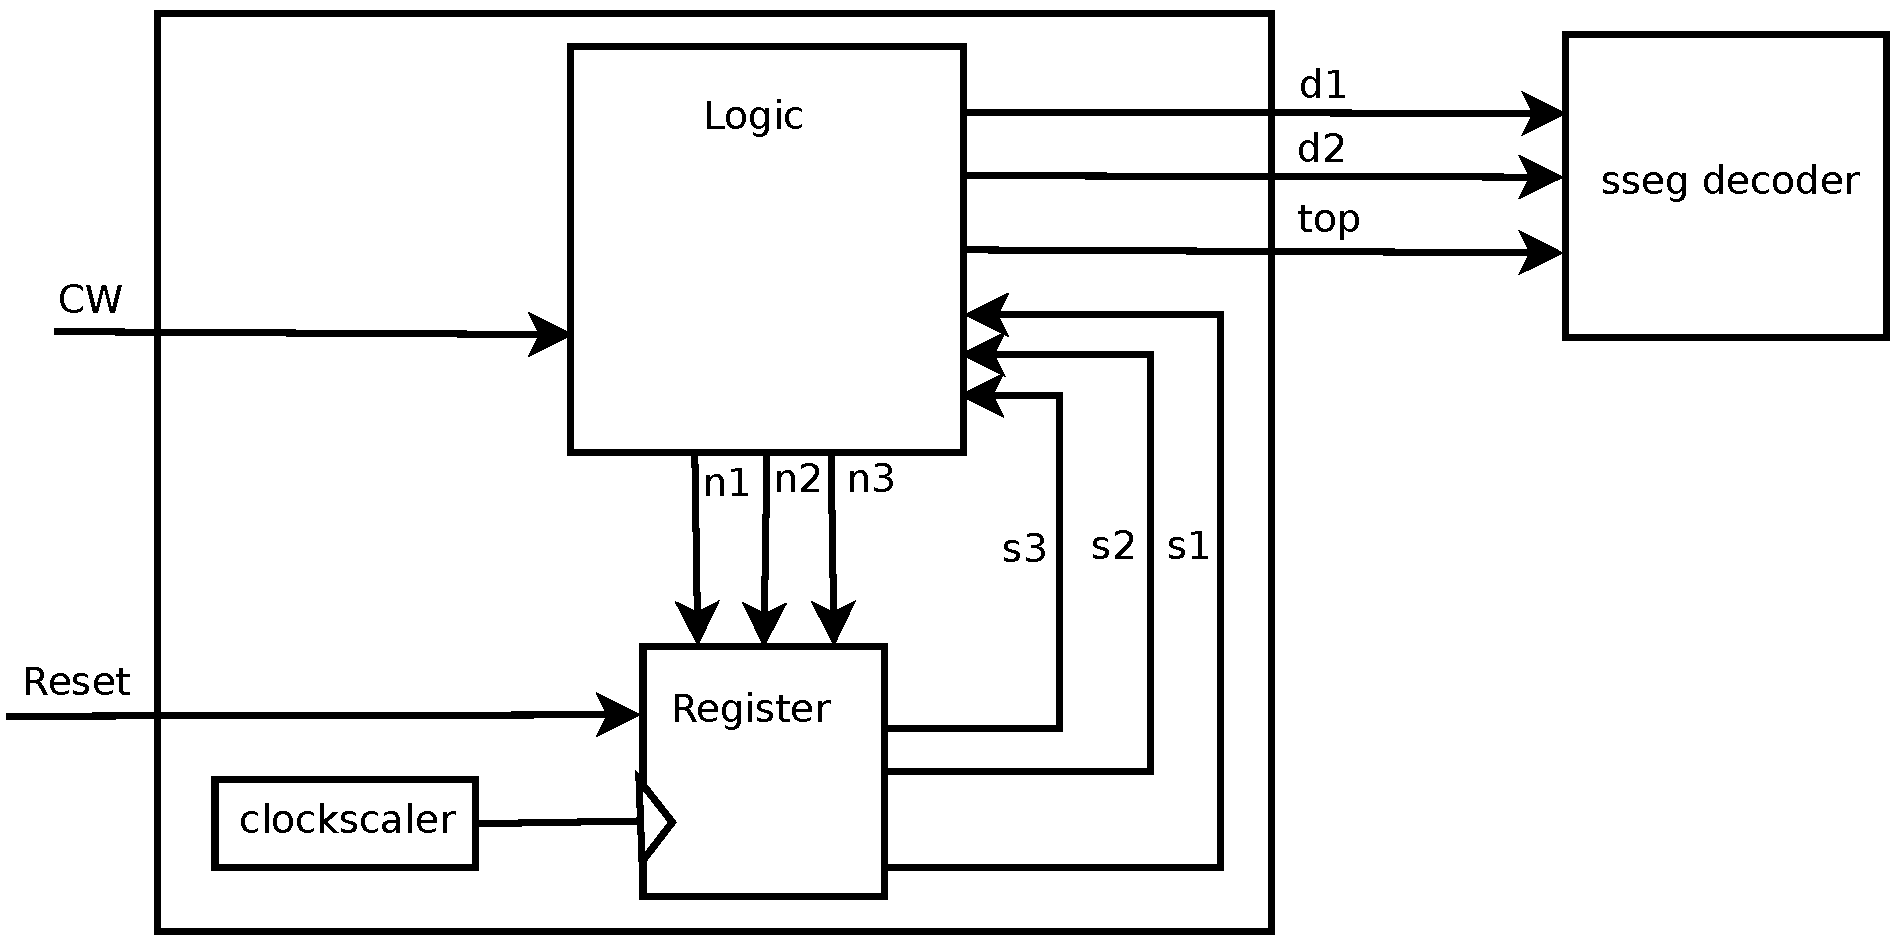
\includegraphics[height=0.4\textwidth]{fig/Block_diagram_implementation.pdf}
	\caption{Block diagram of implementation}
	\label{fig:block_diagram} 
\end{figure}
For making this implementation we have created two new VHDL modules: ``sseg_decoder.vhd'' and ``clockscaler.vhd''. The clockscaler does a downscaling by a factor $10^{6}$ effectively setting the frequency to 5Hz (when having a period of 20ns).\\
The seven segment decoder translates inputs to the physical display.

\subsection{RTL level design}
The RTL level design was created using two muxes instead of combinatorial circuits. The code can be found in ``RTL/Runner_logic.vhd''.